\section{Results: Level 3}\label{sec:results-3}

We begin at level $k=3$, which makes $q=q_3=e^{\frac{2\pi i}{42}}$. 
From the conformal embedding $\hat{\gg_2}\subseteq\hat{\ee_6}$ given in \cite{DMNO} we obtain the 
algebra object $A=V_{\emptyset} \oplus V_{\Lambda_1+\Lambda_2}$, as described in \cite{g2_graphs}. 
Also given in \cite{g2_graphs} is (the orbifold of) the module fusion graph $\Gamma_3$ with adjacency matrix
\[
    M_{\Gamma_3} = \begin{bmatrix} 0&1&1&1\\ 1&1&1&1\\ 1&1&1&1\\ 1&1&1&1\end{bmatrix}.
\]
The graph $\Gamma_3$ itself is depicted on the left side of Figure~\ref{fig:graphs}.

It is known from \cite{DMNO} that 
\[
    \cat{q}_A^0\cong \Vecc(\Z_3);
\]
we deduce from the inclusion $\cat{q}_A^0 \hookrightarrow \cat{q}_A$ that $\cat{q}_A$ contains two $\Z_3$-like simple objects, denoted $g$ and $g^{-1}$. 



\subsection{GPA Embedding and Relations}
Here we give details of both the GPA-embedding of $\DD(q_3)$ and its governing equations. 
Recall that the defining bases \ref{def:GPA} for the spaces 
\[
    \Hom_{\GPA(\Gamma)}(m\to n)
\]
are given in terms of pairs of paths. 
The (undirected) graphs we are using have at most a single edge between any two vertices. 
Hence an edge is equivalent to a pair of vertices, and a path is equivalent to an ordered tuple of vertices. 
For example, the path
\[
    p = v_1 \longrightarrow v_2 \longrightarrow v_3
\]
is equivalent to the ordered triple $(v_1,v_2,v_3)$. 
Which paths $q$ pair validly with $p$ to form a basis element of the $2\to 1$ hom-space of a GPA? 
Well, by definition, $q$ must be parallel to $p$; i.e. the sources and targets of $p$ and $q$ must coincide. 
It follows that the only valid pairing for such $p$ is
\[
    q = v_1 \longrightarrow v_3,
\]
which may also be represented as $(v_1,v_3)$. 
So the only $2\to 1$ basis element which $p$ appears in is
\[
    \big( (v_1,v_2,v_3), (v_1,v_3) \big).
\]
But the parallel condition defining basis elements makes including $(v_1,v_3)$ redundant; we might just as well have called the basis element by 
\[
    (v_1,v_2,v_3).
\]
This is how we refer to $2\to 1$ GPA basis elements. 
Indeed, in Table~\ref{tab:lvl-3-triv-coefs}, the first two columns combine to specify which basis elements are being specified, and the third column gives the approximate coordinate of the trivalent embedding on that basis element. 
For example, the first row of Table~\ref{tab:lvl-3-triv-coefs} tells us that the coordinate of the $(2,2,2)$ basis element is approximately $1.08393$; the second row tells us that the coordinate of the $(4,2,3)$ basis element is approximately $0.619371$. 

Paths of the form $(i,j,i)$, $(i,i,j)$, or $(i,j,j)$ for $i,j\neq1$ require a bit more care to describe. 
There is nontrivial interplay with the graph symmetry swapping vertices 2 and 4. 
When these two vertices are swapped, a path whose coordinate has absolute value $0.155691$ is sent to one whose coordinate has absolute value $1.69414$. 
The nine paths whose coordinates have absolute value $0.155691$ are:
\[
    (2,3,3),\hspace{0.2em} (3,3,2),\hspace{0.2em} (3,2,3),\hspace{0.2em} (2,4,2),\hspace{0.2em} (4,3,4),\hspace{0.2em} (2,2,4),\hspace{0.2em} (3,4,4),\hspace{0.2em} (4,2,2),\hspace{0.2em} (4,4,3) 
\]
One may use symmetry to find the rest of the coordinates.

Table~\ref{tab:lvl-3-proj-coefs} holds numerical approximations to the nonzero projection coordinates. 
There are blocks of nonzero coordinates of length 9 and 16. 
These sizes, and the location of the nonzero real coordinates follow naturally when one considers three facts:
\begin{enumerate}
    \item The object $g$ is $\Z_3$ and simple and therefore has fusion graph given in Figure~\ref{fig:g-fusion-graphs}.
    \item There is a map $T_g \in \Hom_{\cat{q_3}_{A_3}}(Y^{\otimes2} \to g)$ whose outer product $T_g^\dagger \circ T_g$ equals $P_g$, projection onto $g$.
    \item The dagger of a simple projection is itself; i.e., $\left( \skein{/skein_figs/Pg}{0.15} \right)^\dagger = \skein{/skein_figs/Pg}{0.15}$.
\end{enumerate}
The existence and behavior of $T_g$ must be captured by the image of $P_g$ in the GPA, which is all we have access to. This is indeed the case, as the only coordinates of the projection in the GPA which are nonzero are at those basis vectors 
\[
    (i \to\blank\to j, i \to\blank\to j)
\]
where $i\to j$ is a directed edge of the $g$-fusion graph. For $i=j=1$ there are three possible values for $\blank$; pairing them gives 9 pairs. For $i,j\neq 1$ there are four possible values for $\blank$; pairing them gives 16 pairs. The columns of Table~\ref{tab:lvl-3-proj-coefs} give numerical approximations to the coordinates of the projection, with dictionary ordering on the pairs of $\blank$ values. That is, the column labeled by $1\to\blank\to1$ shows the coordinates on the ordered basis
\begin{align*}
    (1\to 2 \to1, 1\to 2 \to1) \\
    (1\to 2 \to1, 1\to 3 \to1) \\
    (1\to 2 \to1, 1\to 4 \to1) \\
    (1\to 3 \to1, 1\to 2 \to1) \\
    (1\to 3 \to1, 1\to 3 \to1) \\
    (1\to 3 \to1, 1\to 4 \to1) \\
    (1\to 4 \to1, 1\to 2 \to1) \\
    (1\to 4 \to1, 1\to 3 \to1) \\
    (1\to 4 \to1, 1\to 4 \to1) \\
\end{align*}
With this ordering and fact (3) above in mind, and recalling that the GPA's dagger operation swaps paths, the real coordinates appear where one would expect them.




% \begin{figure}
%     \centering
%     \includegraphics[width=0.35\linewidth]{figs/graphs/graph_A.png}
%     \includegraphics[width=0.425\linewidth]{figs/graphs/graph_B.png}
%     \caption{Fundamental graphs used for levels 3 (left) and 4 (right).}
%     \label{fig:graphs}
% \end{figure}

\begin{figure}
    \centering
    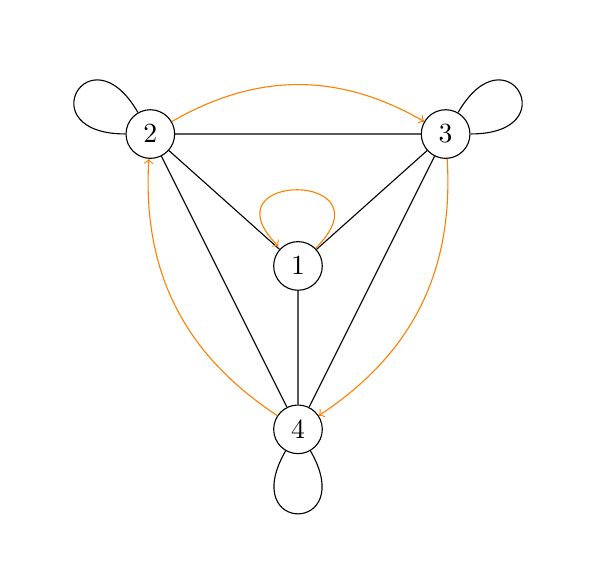
\begin{tikzpicture}[scale=1.25]
        \node[shape=circle,draw=black] (A) at (1.5,1.66) {1};
        \node[shape=circle,draw=black] (B) at (0,3) {2};
        \node[shape=circle,draw=black] (C) at (3,3) {3};
        \node[shape=circle,draw=black] (D) at (1.5,0) {4};
        
        % module fusion graph
        \path (B) edge [loop, in=120, out=180, looseness=10] node {} (B);
        \path (C) edge [loop, in=0, out=60, looseness=10] node {} (C);
        \path (D) edge [loop, in=240, out=300, looseness=10] node {} (D);
        
        \path [-] (D) edge node {} (B);
        \path [-] (B) edge node {} (C);
        \path [-] (C) edge node {} (D);

        \path [-] (A) edge node {} (B);
        \path [-] (A) edge node {} (C);
        \path [-] (A) edge node {} (D);

        % g fusion graph
        \path [->, draw=orange] (B) edge [bend left] node {} (C);
        \path [->, draw=orange] (C) edge [bend left] node {} (D);
        \path [->, draw=orange] (D) edge [bend left] node {} (B);
        \path [->, draw=orange] (A) edge [loop] node {} (A);
    \end{tikzpicture}
    \caption{Fusion graphs at level 3 for $Y$ (black) and $g$ (orange).\\ See \cite[Figure \red{XXX}]{g2_graphs}}
    \label{fig:new-graphs-lvl3}
\end{figure}


\begin{figure}
    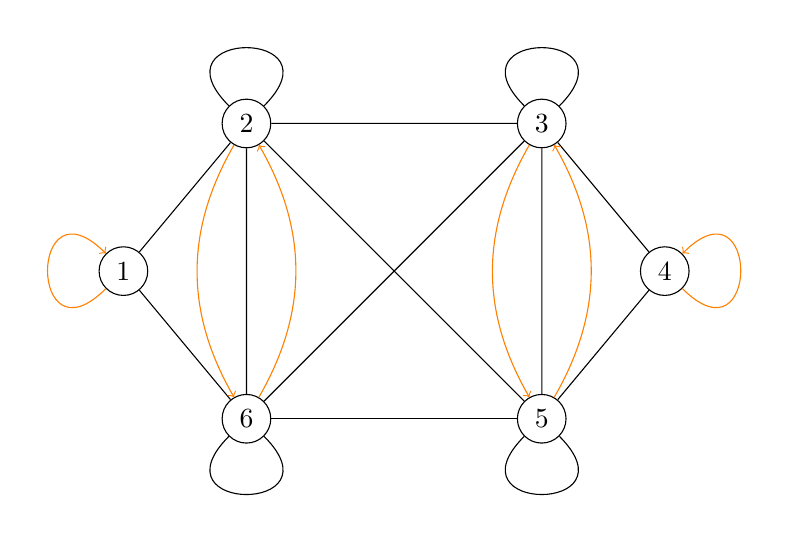
\begin{tikzpicture}[scale=1.25]
        \node[shape=circle,draw=black] (A) at (0,1.5) {1};
        \node[shape=circle,draw=black] (B) at (1.25,3) {2};
        \node[shape=circle,draw=black] (C) at (4.25,3) {3};
        \node[shape=circle,draw=black] (D) at (5.5,1.5) {4};
        \node[shape=circle,draw=black] (E) at (4.25,0) {5};
        \node[shape=circle,draw=black] (F) at (1.25,0) {6};

        % module fusion graph
        \path (B) edge [loop, in=45, out=135, looseness=8] node {} (B);
        \path (C) edge [loop, in=45, out=135, looseness=8] node {} (C);
        \path (E) edge [loop, in=225, out=315, looseness=8] node {} (E);
        \path (F) edge [loop, in=225, out=315, looseness=8] node {} (F);

        \path [-] (A) edge node {} (B);
        \path [-] (A) edge node {} (F);

        \path [-] (B) edge node {} (C);
        \path [-] (B) edge node {} (E);
        \path [-] (B) edge node {} (F);

        \path [-] (C) edge node {} (D);
        \path [-] (C) edge node {} (E);
        \path [-] (C) edge node {} (F);

        \path [-] (D) edge node {} (E);

        \path [-] (E) edge node {} (F);

        % g fusion graph
        \path [->, draw=orange] (A) edge [loop, in=135, out=225, looseness=8] node {} (A);
        \path [->, draw=orange] (D) edge [loop, in=45, out=-45, looseness=8] node {} (D);

        \path [->, draw=orange] (B) edge [bend right] node  {} (F);
        \path [->, draw=orange] (F) edge [bend right] node {} (B);

        \path [->, draw=orange] (C) edge [bend right] node {} (E);
        \path [->, draw=orange] (E) edge [bend right] node {} (C);
    \end{tikzpicture}
    \caption{Fusion graphs at level 4 for $Y$ (black) and $g$ (orange).\\ See \cite[Figure \red{XXX}]{g2_graphs}}
    \label{fig:new-graphs-lvl4}
\end{figure}


\begin{table}
    \centering
    \begin{tabular}{|cc|c|} \hline
        Vertex Path & Conditions & Coefficient \\ \hline\hline
        $(i,i,i)$ &  $i\neq1$ & 1.08393 \\[10pt]  \hline
        $(i,j,k)$ &  $\{i,j,k\}=\{2,3,4\}$   & 0.619371 \\[10pt] \hline
        $(i,1,k)$ &  $i,k\neq 1$, $i\neq k$ & 1.69414 \\[10pt] \hline
        $(i,1,i)$ &  $i\neq 1$   & 0.861006 \\[10pt] \hline
        $(i,i,1)$ or $(1,i,i)$ &  $i\neq1$   & 0.967919 \\[10pt] \hline
    \end{tabular}
    \caption{Level 3 trivalent embedding coefficients.}
    \label{tab:lvl-3-triv-coefs}
\end{table}






\begin{table}
    \centering
    \begin{tabular}{|cccc|} \hline
        $1\to\blank\to1$                    & $2\to\blank\to4$                  & $3\to\blank\to2$               & $4\to\blank\to3$ \\ \hline\hline
        $1.26376$              & $0.791288$                & $0.791288 $              & $0.791288$ \\
        $-0.631881-1.09445 i$   & $0.567622 - 0.684904 i$   & $0.876955 + 0.149123 i$  & $0.674406 + 0.580055 i$ \\
        $-0.631881+1.09445 i$   & $0.674406 + 0.580055 i$   & $0.567622 - 0.684904 i$  & $0.876955 + 0.149123 i$ \\
        $-0.631881+1.09445 i$   & $-0.876955 - 0.149123 i$  & $-0.674406 - 0.580055 i$ & $0.567622 - 0.684904 i$ \\
        $1.26376$               & $0.567622 + 0.684904 i$   & $0.876955 - 0.149123 i$ & $0.674406 - 0.580055 i$ \\
        $-0.631881-1.09445 i$   & $1$                       & $1$                      & $1$ \\
        $-0.631881-1.09445 i$   & $-0.0182917 + 0.999833 i$ & $0.5 - 0.866025 i$       & $0.856735 - 0.515757 i$ \\
        $-0.631881+1.09445i$    & $-0.5 - 0.866025 i$       & $-0.856735 - 0.515757 i$ & $-0.0182917 - 0.999833 i$ \\
        $1.26376$               & $0.674406 - 0.580055 i$   & $0.567622 + 0.684904 i$  & $0.876955 - 0.149123 i$ \\ 
                              & $-0.0182917 - 0.999833 i$ & $0.5 + 0.866025 i$       & $0.856735 + 0.515757 i$ \\
                              & $1$                       & $1$                      & $1$ \\
                              & $-0.856735 + 0.515757 i$  & $0.0182917 - 0.999833 i$ & $0.5 - 0.866025 i$ \\
                              & $-0.876955 + 0.149123 i$  & $-0.674406 + 0.580055 i$ & $0.567622 + 0.684904 i$ \\
                              & $-0.5 + 0.866025 i$       & $-0.856735 + 0.515757 i$ & $-0.0182917 + 0.999833 i$ \\
                              & $-0.856735 - 0.515757 i$  & $0.0182917 + 0.999833 i$ & $0.5 + 0.866025 i$ \\
                              & $1$                       & $1$                      & $1$ \\ \hline
    \end{tabular}
    \caption{Level 3 projection embedding coefficients.}
    \label{tab:lvl-3-proj-coefs}
\end{table}




Finally we give explicit values for the coefficients of the equations of Proposition~\ref{prop:eval-criteria}, excluding (decTetragon) and (decPentagon); the curious reader may find these in the attached Mathematica notebook. The structure constants for $\DD_3$ are:
\begin{equation*}
    \omega = e^{2\pi i/3}
\end{equation*}

\begin{equation*}
    r_1 = ..., \quad r_2 = ..., \quad r_3 = ...
\end{equation*}

\begin{equation*}
    s_1 = ..., \quad s_2 = ..., \quad s_3 = ...
\end{equation*}

\begin{equation*}
    r_1 = ..., \quad r_2 = ..., \quad r_3 = ...
\end{equation*}

\begin{equation*}
    t_1 = ..., \quad t_2 = ..., \quad t_3 = ...
\end{equation*}




\subsection{Theorem and proof}
This subsection is devoted to proving the following theorem.

\begin{theorem}\label{thm:level-3}
    There is a monoidal equivalence
    \[
        \Ab(\ol{\DD_3}) \cong \ol{ \Rep(U_{q_3}(\gg_2))}_{A_3}.
    \]
\end{theorem}

Let $X = V_{\Lambda_1}$ be the object of $\cat{q_3}$ by which we generate the planar algebra $\PP_X \cong \GG_2(q)$. Define $Y=\FF_A(X)$ to be the image of $X$ under the free functor. Now $\FF_{A_3}:\cat{q_3} \to \cat{q_3}_{A_3}$ restricts to an embedding $\PP_{X;\cat{q_3}} \hookrightarrow \PP_{Y;\cat{q}_{A_3}}$. Invertibility of the objects $g$ and $g^{-1}$ implies $g\otimes Y \cong Y$, with rigidity maps for $g$ and $g^{-1}$ building the mutually inverse isomorphisms.

We now compute some important dimensions.
\begin{proposition}\label{prop:level-3-fusion}
    The following are true:
    \begin{enumerate}
        \item $\dim\Hom_{\CC_{A_3}}(Y^{\otimes2}\to Y)=3$
        \item $\dim\Hom_{\CC_{A_3}}(Y^{\otimes2}\to g^k)=1$
        \item $\dim\Hom_{\CC_{A_3}}(Y\to Y)=1$ (i.e., $Y$ is simple)
    \end{enumerate}
\end{proposition}
\begin{proof}
    All three are proved using fusion graph calculations, so we prove only (1)\footnote{See, e.g., Figure 5 of \cite{spectral_measures_G2} for the fusion graph.}. The fusion graph tells us that 
    \[
    V_{\Lambda_1}^{\otimes2} \cong V_\emptyset \oplus V_{\Lambda_1} \oplus V_{2\Lambda_1} \oplus V_{\Lambda_2}
    \]
    and
    \[
    V_{\Lambda_1}\otimes A \cong V_{\Lambda_1} \oplus V_{2\Lambda_1} \oplus  V_{3\Lambda_1} \oplus V_{\Lambda_2} \oplus V_{\Lambda_2+\Lambda_1} \oplus V_{\Lambda_2+2\Lambda_1}.
    \]
    On the other hand, we compute
    \begin{align*}
        \Hom_{\cat{q_3}_{A_3}}(Y^{\otimes2} \to Y) & = \Hom_{\CC_{A_3}}( \FF_{A_3}(V_7)^{\otimes 2} \to \FF_{A_3}(V_7)) \\
        & \cong \Hom_{\cat{q_3}_{A_3}}( \FF_{A_3}(V_7^{\otimes 2}) \to \FF_{A_3}(V_7)) \\
        & = \Hom_{\cat{q_3}_{A_3}}( \FF_{A_3}(V_7^{\otimes 2}) \to V_7\otimes {A_3}) \\
        & \cong \Hom_{\cat{q_3}}( V_7^{\otimes 2} \to V_7\otimes {A_3}). \\
    \end{align*}
    Counting common irreducible constituents of $V_{\Lambda_1}^{\otimes2}$ and $V_{\Lambda_1}\otimes A_3$ gives the desired result.
\end{proof}
We have an immediate consequence.
\begin{corollary}\label{cor:dominant-functor}
        There is a dominant monoidal functor
    \[
        \Psi_3: \DD_3 \to \cat{q}_{A_3}
    \]
    which maps 
    \[
        \skein{/skein_figs/trivalent}{0.15} \mapsto \tau\in\Hom_{\cat{q_3}_{A_3}}(Y^{\otimes2}\to Y), \quad \skein{/skein_figs/Pg}{0.15} \mapsto P_g \in\End_{\cat{q_3}_{A_3}}(Y^{\otimes2})
    \]
\end{corollary}
\begin{proof}
    Proposition~\ref{prop:level-3-fusion}, along with the defining relations of $\DD_3$ tell us this assignment is functorial. 
    Since $Y$ is a $\otimes$-generator and $\Psi_3$ surjects onto objects of $\PP_Y$, dominance also follows.
\end{proof}




\begin{lemma}\label{lem:faithful}
    The induced map
    \[
        \ol{\Psi_3} : \ol{\DD_3} \to \ol{\Rep(U_{q_3}(\gg_2))}_{A_3} 
    \]
    is faithful.
\end{lemma}
% Why do we care...?
\begin{proof}
    The evaluation algorithm for $\DD_3$ implies that $\DD_3$ has simple unit. Therefore every ideal is contained in the ideal of negligibles, which is killed when passing to the semisimplification $\ol{\DD}$. Hence the map $\ol{\Psi_3}$ has no kernel.
\end{proof}

\begin{comment}
    
\begin{proof}[Proof of Theorem~\ref{thm:level-3}]
    We now note that since $\GG_2(q)$ and $\DD_3$ are unitary, we know that $\GG_2(q) \hookrightarrow \DD_3$ induces a $\dagger$-embedding $\ol{\GG_2(q)} \hookrightarrow \ol{\DD_3}$. Thus, there is a chain
    \[
        \ol{\GG_2(q_3)} \hookrightarrow \ol{\DD_3} \xhookrightarrow{\ol{\Psi_3}} \ol{\Rep(U_{q_3}(\gg_2))}_{A_3}
    \] 
    of faithful dominant functors. Using the universal property of Karoubi completion, we arrive at the commutative diagram
    \[
        \xymatrix@R=40pt@C=65pt{
        \ol{\GG_2(q_3)} \ar@{^{(}->}[r] \ar@{^{(}->}[d] & \ol{\DD_3} \ar@{^{(}->}[dr]^{\ol{\Psi}} \ar@{^{(}->}[d] & \\
        \ol{\Rep(U_{q_3}(\gg_2))} \ar[r]^{\FF_1} & \Ab(\ol{\DD_3}) \ar[r]^{\FF_2} & \ol{\Rep(U_{q_3}(\gg_2))}_{A_3} \\
        }
    \]
    where $\FF_1$ and $\FF_2$ are the induced functors. At this point we shift our focus to the lower layer of the diagram.
    
    By \cite{},  $(\FF_2 \circ \FF_1)|_{\ol{\GG_2(q_3)}} = \FF_{A_3}|_{\ol{\GG_2(q_3)}}$ implies $\FF_2 \circ \FF_1 = \FF_{A_3}$. 
    Note that both $\ol{\Rep(U_{q_3}(\gg_2))}$ and $\Ab(\ol{\DD_3})$ are semisimple, and therefore $\FF_1$ has a lax-monoidal right adjoint $\FF_1^\vee$. 
    Proposition~\ref{prop:exact-functor} now allows us to conjure $K$ and $B$ such that the following diagram commutes up to natural isomorphism:
    \[
        \xymatrix@R=40pt@C=65pt{
        \ol{\Rep(U_{q_3}(\gg_2))} \ar[r]^{\FF_1} \ar[dr]_{\FF_B} & \Ab(\ol{\DD_3}) \ar[r]^{\FF_2} \ar[d]^{K} & \ol{\Rep(U_q(\gg_2))}_A \\
        & \ol{\Rep(U_q(\gg_2))}_B \ar[ur]_{\FF'} & \\
        }
    \]
    Here, $\FF'$ is defined to complete the diagram. From here, apply $\FF_B^\vee$ to the containment $\unit \subseteq \FF'^\vee(\unit)$:
    \begin{align*}
        B & = \FF_B^\vee(\unit) \subseteq \FF_B^\vee \circ \FF'^\vee(\unit) \\
        & \cong (\FF_2 \circ \FF_1)^\vee (\unit) \\
        & = \FF_{A_3}^\vee(\unit) \\
        & = \FF_A^\vee(A_3) = A_3.
    \end{align*}
    
    So $B\subseteq A_3$. Since $A_3$ has only two simple summands, we know $A_3$ has no nontrivial subalgebras: $B\cong \unit$ or $B\cong A_3$.
    If $B\cong \unit$ then
    \[
        \Ab(\ol{\DD_3}) \cong \ol{\Rep(U_{q_3}(\gg_2))}_\unit \cong \ol{\Rep(U_{q_3}(\gg_2))}
    \]
    A quick dimension count falsifies this. Hence $\Ab(\ol{\DD_3}) \cong \ol{ \Rep(U_{q_3}(\gg_2))}_{A_3}$.
\end{proof}

\end{comment}






\section{Results: Level 4}\label{sec:results-4}
At level $k=4$ we have $q = q_4 = e^{\frac{2\pi i}{48}}$ and 
$A_4=V_\emptyset \oplus V_{3\Lambda_1}$. 
From \cite{DMNO} we have $\cat{q_4}_{A_4}^0 \cong \Vecc(\Z_2)$, giving us one new 
$\Z_2$-like simple object $h$. 
The module fusion graph for level 4 is show in Figure~\ref{fig:new-graphs-lvl4}
The details of the GPA embedding at level 4 are less instructive than the level 3 case, 
so we relegate the details to the attached Mathematica files. 
Much of the story remains the same. 
The trivalent coordinates are algebraically nicer than those at level 3; 
up to sign, we showed 5 of 9 in Subsection~\ref{subsec:triv-vertex}. 
The nonzero coordinates of the projection come in blocks of \red{4, and 9}. 
There is also an analogue of Theorem~\ref{thm:level-3} for level 4.

\begin{theorem}\label{thm:level-4}
    There is a monoidal equivalence
    \[
        \Ab(\ol{\DD(q_4)}) \cong \ol{ \Rep(U_{q_4}(\gg_2))}_{A_4}.
    \]
\end{theorem}

This theorem is proved by using analogues of Proposition~\ref{prop:level-3-fusion}, Corollary~\ref{cor:dominant-functor}, Lemma~\ref{lem:faithful}.
The same argument used in the proof of Theorem~\ref{thm:level-3} except with, e.g., every $q_3$ switched out for a $q_4$, may be applied.

Note that since $\cat{q_4}_{A_4}^0$ contributes a $\Z_2$-like simple object, there is only one decoration of a trivalent vertex;
we represent this as an undirected colored strand.
The structure constants for $\DD_4$ are:
\begin{equation*}
    \omega = -1
\end{equation*}

\begin{equation*}
    r_1 = e^{-\frac{\pi i}{6}}, \quad r_2 = e^{-\frac{2\pi i}{3}}
\end{equation*}

\begin{equation*}
    s_1 = e^{-\frac{\pi i}{6}} \quad s_2 = e^{-\frac{4\pi i}{3}}
\end{equation*}

\begin{equation*}
    t_1 = -1 \quad t_2 = -1
\end{equation*}

